\chapter{Interfaces De Usuario}
\label{capitulotres}

Dentro de este cap'itulo se hablar'a sobre algunas caracter'isticas importantes que se tienen que tomar en cuenta para el dise\~no de interfaces de usuario y algunas t'ecnicas que se utilizan para fundamentar el desarrollo del trabajo de grado.

\section{Interfaz De Usuario}
Se puede definir a la interfaz de usuario como el elemento encargado de permitir la comunicaci'on del usuario con la m'aquina o el sistema. Dada esta definici'on, necesitamos describir dos elementos importantes para poder entender mejor a una interfaz de usuario:

\begin{itemize}
	\item Elementos de entrada: Elementos  de informaci'on ingresados por el usuario, como ser: 'ordenes, comandos o cualquier otro elemento que el usuario pueda ingresar como pauta de lo que quiere conseguir.

	\item Elementos de salida: Son los elementos obtenidos de las acciones ejecutadas por el usuario, que acercan al mismo a obtener lo que espera y lograr así su meta.
\end{itemize}

\medskip
Las interfaces de usuario se pueden clasificar en tres tipos: F'isicas, Gr'aficas, y Tangibles. Los cuales son descritos brevemente a continuaci'on.

\begin{itemize}
	\item \textbf{PUI (\textit{Physical User Interface} - Interfaz de usuario f'isica):} Son las interfaces de usuario f'isicas, generalmente presentes en maquinaria, autos, u otros, son los medios mec'anicos mediante los cuales un usuario puede comunicarse con un sistema determinado.
 
	\item \textbf{ GUI (\textit{Graphical User Interface} - Interfaz de usuario gr'afica):} Son las interfaces gr'aficas generalmente presentes en sistemas computacionales o sistemas digitales, constan de elementos gr'aficos (botones, texto, im'agenes, etc.) dentro de una pantalla en el computador.

	\item \textbf{TUI (\textit{Tangible User Interface} - Interfaz de usuario tangible):} Las Interfaces de usuario tangibles emplean objetos reales para representaci'on y control en un medio computacional. Este tipo de interfaz de usuario est'a presente generalmente en sistemas de entrenamiento o simulaci'on, donde por ciertos motivos no se puede interactuar con un sistema real pero se intenta que la experiencia del usuario sea lo m'as parecida a ella.
\end{itemize}

\medskip
Las GUI han ido evolucionando de la mano de la tecnolog'ia, podemos ver claramente esto en su historia, cuando se pas'o de un texto plano siendo ejecutado como 'ordenes al computador, a un elemento visual orientado a satisfacer distintos tipos de necesidades de los usuario. Con la evoluci'on tambi'en se generaron criterios que nos permiten diferenciar la calidad de las GUI, permitiendo de esta manera un mayor desarrollo y aprovechamiento de este elemento tan importante.
Entre dichos criterios sobresalen enormemente dos, que son: la usabilidad  y la naturalidad.

\subsection{Usabilidad}
La usabilidad, es una caracter'istica muy importante para obtener la aprobaci'on del usuario en cualquier sistema, la misma se define como el elemento que mide el grado en el que el usuario puede realizar sus actividades, mientras más sencillo le resulte al usuario realizar sus actividades m'as usable ser'a la interfaz, por ende m'as usable ser'a el sistema. 
La usabilidad abarca dos conceptos fundamentales:

\begin{itemize}
	\item \textbf{Funcionalidad:} Que se refiere a las caracter'isticas del sistema que permiten al usuario realizar sus tareas.

	\item \textbf{Facilidad de uso:} Se provee caracter'isticas para que el sistema sea más f'acil de aprender y permite realizar tareas m'as f'acilmente.

\end{itemize}

\medskip
Cuando se usa el t'ermino usabilidad los programadores se enfocan especialmente en el primer concepto, dejando de lado factores esenciales como la experiencia del usuario cuando intenta usar el sistema, se olvida preguntarse, ¿el usuario puede encontrar lo que busca?, ¿El sistema le permite realizar su trabajo m'as f'acil?
Se puede decir que la usabilidad consiste de seis factores los cuales son presentados a continuaci'on:

\begin{itemize}
	\item \textbf{ Apto para el uso (Funcionalidad): } El sistema soporta las tareas que tienen los usuarios en la vida real.
	
	\item \textbf{F'acil de Aprender:} El sistema es f'acil de usar para distintos grupos de usuarios.

	\item \textbf{Eficiencia en las Tareas:} Cuan eficiente es el sistema para los usuarios frecuentes.

	\item \textbf{F'acil de Recordar:} Cuan f'acil de recordar es para los usuarios ocasionales.

	\item \textbf{Satisfacci'on Subjetiva:} Cu'an satisfecho est'a el usuario con el sistema.
	
	\item \textbf{Entendible:} Cu'an f'acil es entender lo que el sistema est'a haciendo. Este factor es muy importante en ciertas ocasiones como ser fallas del sistema o errores.
\end{itemize}

\medskip

\subsection{Naturalidad}
La naturalidad es una caracter'istica que se enfoca m'as a cu'an natural es para el usuario realizar sus actividades, por ejemplo los usuarios en general est'an acostumbrados a salir de los programas mediante un bot'on en una de las esquinas superiores de la ventana, dicho bot'on est'a representado por una x, cambiar esto podr'ia significar un choque con lo que el usuario conoce, esto le restar'ia naturalidad a la interface que se est'a desarrollando, por lo tanto lo que se intenta con esta caracter'istica es presentarle al usuario elementos que ya conoce para poder estimular su memoria y facilitar su trabajo, pues se dice que la memoria es la forma m'as simple de inteligencia.
Dadas las anteriores definiciones podemos continuar describiendo el proceso de dise\~no de una interfaz de usuario con algunas heur'isticas para lograr un mejor resultado.

\section{Dise\~no de interfaces gr'aficas de usuario}
Soren Lauesen \cite{lauesen2005user} sostiene que, si consultamos a un programador sobre la interfaz de usuario, el responde que es un elemento sencillo, que se puede realizar despu'es de haber concluido las tareas m'as importantes del sistema, en cambio si trasladamos la misma pregunta al dise\~nador de interfaces, este nos dice que es uno de los elementos m'as importantes dentro del desarrollo de un proyecto, y que por ende debe realizarse antes que las dem'as tareas, y en participaci'on con programadores, clientes, dise\~nadores y otros.
Podemos evidenciar que se tienen puntos de vista diferentes, y se puede afirmar que ambos tienen algo de raz'on, hacer una interfaz de usuario es una tarea relativamente sencilla, pero hacer una interfaz de usuario que agrade al cliente es ya una tarea mucho m'as complicada.
Existen diversas t'ecnicas que pueden ser usadas dentro del dise\~no de interfaces una de las m'as importantes y la que se tratara a lo largo de este art'iculo es el sketch (prototipado) y sus ventajas.

\subsection{Sketch Design}

Sketch es una t'ecnica de dise\~no muy ventajosa en diversos aspectos, este m'etodo de dise\~no se basa esencialmente en el prototipado.
	El prototipado es una pr'actica muy usada en el 'ambito de la arquitectura, por el costo que implica no se puede realizar pruebas reales en las que las personas puedan caminar, as'i que se realizan modelos en papel, maquetas, planos, etc. Para permitir que el o los usuarios puedan opinar sobre el producto antes de que  el mismo est'e terminado, esta pr'actica es muy 'util a la hora de ahorrar tiempo y dinero. El sketch modeling se basa en desarrollar modelos mediante dibujos de la interfaz de usuario.
¿Por qu'e realizar prototipos?
Los prototipos son f'aciles y r'apidos de desarrollar, f'aciles de cambiar y f'aciles de desechar, permite ahorrar tiempo y dinero, permite contar con diferentes alternativas, solucionar problemas antes de que el c'odigo sea escrito y mantener el enfoque del dise\~no en el usuario.
El prototipado de una interfaz de gr'afica puede tener diversos tipos de fidelidad, la fidelidad de un prototipo se mide de acuerdo al nivel de detalle que se us'o al momento de realizar el prototipo, existen 3 niveles de fidelidad: low fidelity, m'edium fidelity, high fidelity. 

\begin{itemize}
	\item \textbf{Low Fidelity}
	Son los prototipos de fidelidad baja, que son llamados trazos art'isticos, el prototipo est'a formado por dibujos simples y de baja representaci'on, como se muestra en la siguiente figura \ref{fig:LowFidelity}.

\begin{figure}[ht]
    \centering
    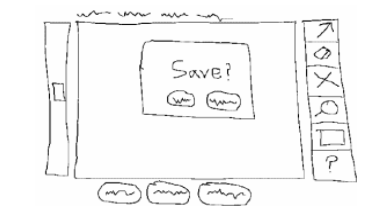
\includegraphics[width=0.75\textwidth]{Figura0301LowFidelity}
    \caption{Ejemplo de un prototipo de baja fidelidad.}
    \label{fig:LowFidelity}
\end{figure}
\medskip

	\item \textbf{Medium Fidelity}
	Los prototipos de fidelidad media son prototipos con una semejanza mayor a los modelos reales, aunque siguen siendo dibujos estos dibujos poseen un nivel mayor de semejanza y detalle. En la Figura \ref{fig:MediumFidelity} se muestra un ejemplo de un prototipo de fidelidad media.
	
\begin{figure}[ht]
    \centering
    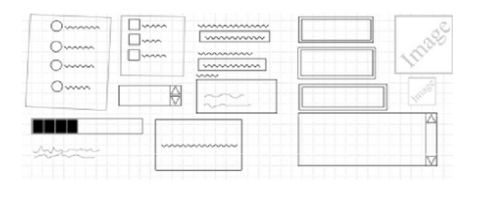
\includegraphics[width=0.75\textwidth]{Figura0302MediumFidelity}
    \caption{Ejemplo de un prototipo de fidelidad media.}
    \label{fig:MediumFidelity}
\end{figure}

	\item \textbf{High Fidelity}
	Son prototipos de una calidad m'as elevada, constan de un parecido mucho mayor a lo que se quiere representar, su detalle es mucho m'as alto por ende es m'as representativo. En la figura \ref{fig:HighFidelity} podemos apreciar un ejemplo de prototipo de  alto nivel de fidelidad.

\begin{figure}[ht]
    \centering
    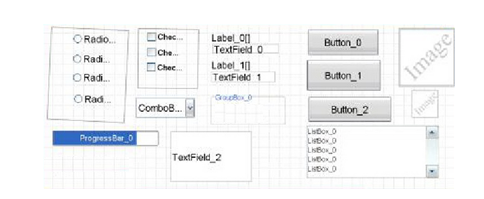
\includegraphics[width=0.75\textwidth]{Figura0303HighFidelity}
    \caption{Ejemplo de un prototipo de fidelidad alta.}
    \label{fig:HighFidelity}
\end{figure}	
\end{itemize}

El presente proyecto plantea realizar un sistema colaborativo para el dise\~no de interfaces de usuario mediante prototipos en alta fidelidad, de esta manera permitir a los usuarios ver el resultado m'as aproximado al resultado final.